% Compile with XeLaTeX.
% Faithful transcription of supplied photographs, pp. 160--162, section 7.1.2.
% Paragraph identifiers [28]--[42] continue the existing notes.
\documentclass[11pt,a4paper,twoside]{article}

\usepackage{fontspec}



\IfFontExistsTF{Times New Roman}{\setmainfont{Times New Roman}}{\setmainfont{Latin Modern Roman}}



\usepackage{amsmath,amssymb,mathtools,empheq}



\usepackage{tikz,wrapfig}

\usepackage[a4paper,inner=2.5cm,outer=2cm,top=2.5cm,bottom=2.5cm]{geometry}

\usepackage{setspace}

\setstretch{1.25}

\setlength{\parindent}{2em}

\setlength{\parskip}{5pt}

\setlength{\abovedisplayskip}{6pt}

\setlength{\belowdisplayskip}{6pt}

\setlength{\abovedisplayshortskip}{4pt}

\setlength{\belowdisplayshortskip}{4pt}

\usepackage{fancyhdr}

\usepackage[hang,flushmargin]{footmisc}

\pagestyle{fancy}

\fancyhf{}

\renewcommand{\headrulewidth}{0pt}

\fancyfoot[RO,LE]{\small $\boldsymbol{\cdot}\;\thepage\;\boldsymbol{\cdot}$}

\newcommand{\pnum}[1]{\makebox[0pt][r]{\scriptsize\textbf{[#1]}\hspace{0.7em}}}


% Traditional Chinese review notes; compile with XeLaTeX.
\usepackage{xeCJK}
\IfFontExistsTF{DFKai-SB}{\setCJKmainfont{DFKai-SB}}{%
  \IfFontExistsTF{Noto Serif CJK TC}{\setCJKmainfont{Noto Serif CJK TC}}{%
    \IfFontExistsTF{Noto Serif TC}{\setCJKmainfont{Noto Serif TC}}{%
      \setCJKmainfont{FandolSong-Regular}}}}
\usepackage[most]{tcolorbox}
\newtcolorbox{studyNote}[1]{enhanced,breakable,
  colback=gray!4,colframe=black!35,boxrule=0.5pt,arc=1mm,
  left=2mm,right=2mm,top=1.5mm,bottom=1.5mm,
  before skip=8pt,after skip=8pt,fonttitle=\bfseries,title={#1}}
\newcommand{\StudyNote}[2]{\begin{studyNote}{#1}#2\end{studyNote}}

\begin{document}


% Original page 160: section 7.1.2 begins.
\noindent{\large\bfseries 7.1.2\quad Fermat's Principle}
\par\vspace{0.6em}\hrule\vspace{0.8em}
\noindent\pnum{28}Ultimately, all fundamental laws of physics can be expressed using the calculus of variations. One of the first examples was a suggestion by Fermat, in 1662, that a light ray travels the path that takes the least time. This is known as \textit{Fermat's principle}.

\noindent\pnum{29}For a light ray moving in a vacuum, Fermat's principle just reaffirms
% Original page 161: continuation of paragraph [29].
the obvious statement that light travels in a straight line between any two points. But things become more interesting when we consider light travelling in some material, where it no longer travels at speed $c$, but instead at the lower speed $v=c/n$ where $n$ is called the \textit{refractive index}.

% Vector reconstruction of the unnumbered source figure.
\begin{wrapfigure}{r}{0.38\textwidth}
    \centering
    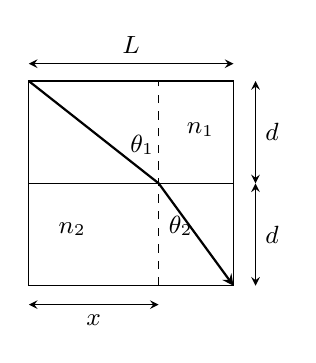
\begin{tikzpicture}[x=1cm,y=1cm,>=stealth,font=\small]
        \draw (0,0) rectangle (2.6,2.6);
        \draw (0,1.3)--(2.6,1.3);
        \draw[dashed] (1.65,0)--(1.65,2.6);
        \draw[->,thick] (0,2.6)--(1.65,1.3)--(2.6,0);
        \draw[<->] (0,2.82)--(2.6,2.82) node[midway,above] {$L$};
        \draw[<->] (0,-.24)--(1.65,-.24) node[midway,below] {$x$};
        \draw[<->] (2.88,1.3)--(2.88,2.6) node[midway,right] {$d$};
        \draw[<->] (2.88,0)--(2.88,1.3) node[midway,right] {$d$};
        \node at (2.18,1.98) {$n_1$};
        \node at (.55,.72) {$n_2$};
        \node at (1.44,1.79) {$\theta_1$};
        \node at (1.93,.76) {$\theta_2$};
    \end{tikzpicture}
\end{wrapfigure}
\noindent\pnum{30}Suppose that a light ray moves between two different materials, the first with an index of refraction $n_1$, the second with $n_2$ as shown in the figure. The light ray travels a total distance $L$ in the horizontal direction, and a distance $2d$ in the vertical direction, but we suppose that it has a choice about the point $x$ where it transitions from one material to the other. We can think of the total time taken $T$ to be a function of $x$: it is
\[
    T(x)=\frac{\sqrt{d^2+x^2}}{v_1}
    +\frac{\sqrt{d^2+(L-x)^2}}{v_2}.
\]
\noindent\pnum{31}To minimize this, we don't need any fancy calculus of variations. We just need to differentiate
\begin{equation}
    \frac{dT}{dx}=\frac{x}{v_1\sqrt{d^2+x^2}}
    -\frac{L-x}{v_2\sqrt{d^2+(L-x)^2}}=0.
    \tag{7.20}
\end{equation}

% Protocol 2: review note 1.
\StudyNote{複習註解一：為什麼（7.20）要令 $dT/dx=0$？}{
起點與終點固定時，改變光線穿過介面的位置 $x$，就會改變兩段路程及總時間 $T(x)$。依費馬原理，本例要找出使總時間最小的交會位置。

若某位置滿足 $T'(x)\neq0$，就能選擇向左或向右微調 $x$，使時間減少，因此該位置不會是極小值。故極小值必須滿足
\[
    T'(x)=0,
\]
這就是（7.20）的由來：交會點微小移動時，第一段增加的時間與第二段減少的時間在一階近似下恰好抵銷。

單憑 $T'(x)=0$ 只能判定駐點；本例另有
\[
    T''(x)=
    \frac{d^2}{v_1(d^2+x^2)^{3/2}}
    +\frac{d^2}{v_2[d^2+(L-x)^2]^{3/2}}>0,
\]
所以此駐點確實給出最小時間。一般而言，費馬原理要求的是時間取駐值。
}

\noindent\pnum{32}This has a nice geometrical interpretation in terms of the angles shown in the figure: we have
\begin{equation}
    \frac{\sin\theta_1}{v_1}=\frac{\sin\theta_2}{v_2}
    \quad\Longrightarrow\quad n_1\sin\theta_1=n_2\sin\theta_2.
    \tag{7.21}
\end{equation}
\noindent\pnum{33}This is \textit{Snell's law} for refraction.

\noindent\pnum{34}In more complicated situations, Fermat's principle gives a problem that falls very much in the camp of calculus of variations. Suppose that light moves in the $(x,y)$-plane with the refractive index varying continuously as $n(y)$. An example of this happens for the air above a hot, shimmering road, where refraction causes a \textit{mirage} to appear as light from the sky bends.

\noindent\pnum{35}We consider light travelling from $(x,y)=(a,A)$ to $(x,y)=(b,B)$. The time taken along a general path $y(x)$ is given by
\begin{equation}
    T=\frac{1}{c}\int_a^b dx\ n(y)\sqrt{1+y'(x)^2}.
    \tag{7.22}
\end{equation}

% Protocol 2: review note 2.
\StudyNote{複習註解二：（7.22）如何表示光沿曲線行進的時間？}{
    $y(x)$ 描述從 $(a,A)$ 到 $(b,B)$ 的一條候選光路；折射率 $n(y)$ 隨高度改變，因此當地光速為
    \[
        v(y)=\frac{c}{n(y)}.
    \]
    書中的例子是熱路面上方的空氣，但公式也適用於其他具有折射率分布 $n(y)$ 的介質。

    沿路徑由左往右取一小段，其弧長與所需時間分別為
    \[
        ds=\sqrt{dx^2+dy^2}=\sqrt{1+y'(x)^2}\,dx,
        \qquad
        dt=\frac{ds}{v(y)}=\frac{n(y)}{c}\,ds.
    \]
    把各小段的時間累加，即得
    \[
        T[y]=\frac1c\int_a^b n(y(x))\sqrt{1+y'(x)^2}\,dx.
    \]
    \textbf{（7.22）計算的是沿指定路徑行進的時間，尚未決定實際光路。}
    接下來才對路徑作變分，利用費馬原理求出光所走的路徑。
}


\newpage
% Original page 162.
\noindent\pnum{36}The Euler--Lagrange equation is
\begingroup\small
\begin{equation}
    \frac{\partial L}{\partial y}-\frac{d}{dx}\left(\frac{\partial L}{\partial y'}\right)
    =\sqrt{1+y'(x)^2}\,\frac{\partial n}{\partial y}
    -\frac{d}{dx}\left(\frac{n(y)y'(x)}{\sqrt{1+y'(x)^2}}\right)=0.
    \tag{7.23}
\end{equation}
\endgroup
\noindent\pnum{37}That's rather a mess. But there is, it turns out, a hidden simplification. You can show that the Euler--Lagrange equation (7.23) implies that
\begin{equation}
    \frac{n(y)}{\sqrt{1+y'^2}}=\text{constant}.
    \tag{7.24}
\end{equation}

% Protocol 2: review note 3.
\StudyNote{複習註解三：如何由（7.23）得到（7.24）？}{
    令 $n_y=dn/dy$。因為 $n=n(y(x))$，由鏈鎖律，
    \[
        \frac{dn}{dx}=n_y y'.
    \]
    因此
    \[
        \frac{d}{dx}\left(\frac{ny'}{\sqrt{1+y'^2}}\right)
        =\frac{n_y y'^2}{\sqrt{1+y'^2}}
        +\frac{ny''}{(1+y'^2)^{3/2}}.
    \]
    代回（7.23）並合併前兩項，可得
    \[
        \frac{n_y}{\sqrt{1+y'^2}}
        -\frac{ny''}{(1+y'^2)^{3/2}}=0,
    \]
    亦即
    \[
        \boxed{n_y(1+y'^2)-ny''=0.}
    \]
    接著，對（7.24）左邊微分：
    \[
        \begin{aligned}
            \frac{d}{dx}\left(\frac{n}{\sqrt{1+y'^2}}\right)
             & =\frac{n_y y'}{\sqrt{1+y'^2}}
            -\frac{ny'y''}{(1+y'^2)^{3/2}}   \\
             & =\frac{y'}{(1+y'^2)^{3/2}}
            \underbrace{\left[n_y(1+y'^2)-ny''\right]}_{=\,0}.
        \end{aligned}
    \]
    故其導數為零，得到
    \[
        \boxed{\frac{n(y)}{\sqrt{1+y'^2}}=\text{constant}.}
    \]
    \textbf{這表示沿著滿足 Euler--Lagrange 方程的光路，折射率 $n(y)$ 與斜率 $y'$ 雖可改變，但上述比值保持不變。}
    推導過程沒有除以 $y'$，所以在 $y'=0$ 的位置也適用。

    這個組合也有系統性的來源：當 $L$ 沒有顯含 $x$ 時，沿著 Euler--Lagrange 方程的解，$L-y'\partial L/\partial y'$ 為常數。本例
    \[
        \begin{aligned}
            L-y'\frac{\partial L}{\partial y'}
             & =n\sqrt{1+y'^2}-\frac{ny'^2}{\sqrt{1+y'^2}} \\
             & =\frac{n}{\sqrt{1+y'^2}},
        \end{aligned}
    \]
    正好就是（7.24）的左邊。
}

\noindent\pnum{38}Showing this directly is straightforward, but laborious: just use the chain rule to get an explicit expression for that $d/dx$ term in the Euler--Lagrange equation (7.23) and then show that the same Euler--Lagrange equation appears when you differentiate the combination $n(y)/\sqrt{1+y'^2}$. Later in this chapter, we'll give a more direct way to see why (7.24) is constant. (It is related to the conservation of energy in classical mechanics.)

\noindent\pnum{39}For a given profile $n(y)$, we can go ahead and solve (7.24). For example, we take the refractive index to be
\begin{equation}
    n(y)=\sqrt{a-by}.
    \tag{7.25}
\end{equation}
\noindent\pnum{40}Then (7.24) becomes
\begin{equation}
    \frac{a-by}{1+y'^2}=k^2
    \quad\Longrightarrow\quad
    y'(x)^2=\frac{b}{k^2}\bigl(y_0-y(x)\bigr).
    \tag{7.26}
\end{equation}
\noindent\pnum{41}Here $k$ is the constant on the right-hand side of (7.24) and $y_0=(a-k^2)/b$. The solution to this equation is
\begin{equation}
    y(x)=y_0-\frac{b}{4k^2}(x-x_0)^2.
    \tag{7.27}
\end{equation}
\noindent\pnum{42}We see that, with the refractive index (7.25), light doesn't travel in a straight line at all. Instead, it travels in a parabola! That's rather striking, not least because a ball thrown under the influence of gravity also travels in a parabola. It might make you wonder if perhaps we can phrase more general mechanics problems in a similar way. And, indeed, we can. Although, as we'll see shortly, it's typically not the time that we want to minimise.
% End of section 7.1.2. No text from section 7.1.3 is included.

\end{document}